\chapter{Los plásticos y los materiales sintéticos}\label{ch:g8:plastics}

Cuenta los objetos de \omterm{def:g8:plastics:plastic}{plástico} que tocas en una mañana: un cepillo de
dientes, una botella, un impermeable, una funda de móvil, el asiento de
un autobús, la bolsa de la compra. Casi ninguno existía hace ciento
veinte años, y ninguno ha crecido en un árbol ni se ha extraído del
suelo. Los \omterm{def:g8:plastics:plastic}{plásticos} son materiales inventados por los químicos
(ligeros, baratos, impermeables, se les puede dar cualquier forma), y
ese mismo éxito se ha convertido en un problema.

\begin{recall}
Los \omterm{def:g5:raw-materials-and-recycling:natural-material}{materiales naturales} se usan casi tal como se encuentran en la
naturaleza; los \omterm{def:g5:raw-materials-and-recycling:natural-material}{materiales elaborados} se fabrican a partir de \omterm{def:g5:raw-materials-and-recycling:raw-material}{materias
primas} transformándolas, y el \omterm{def:g5:raw-materials-and-recycling:recycling}{reciclaje} convierte el material de los
objetos viejos en objetos nuevos
(\cref{ch:g5:raw-materials-and-recycling}). La \omterm{def:g4:what-a-fire-needs:burning}{combustión} de un
\omterm{def:g4:what-a-fire-needs:fuel}{combustible} formado por carbono e hidrógeno da dióxido de carbono y agua
(\cref{ch:g8:combustion-and-fuels}).
\end{recall}

\begin{omfigure}
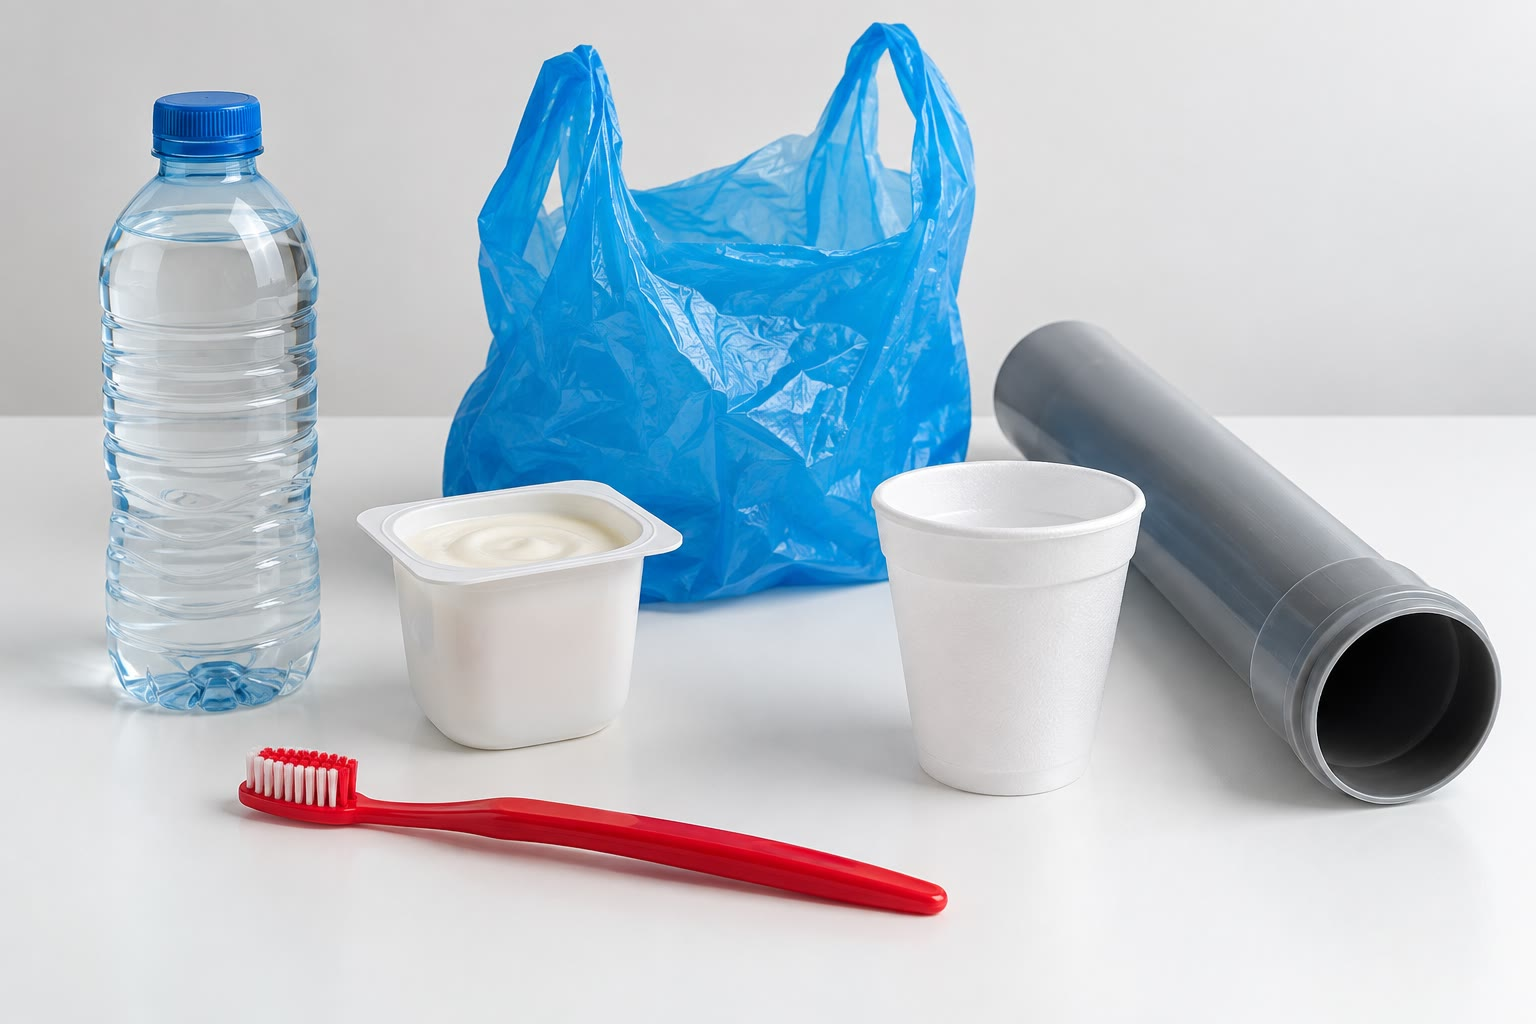
\includegraphics[width=0.55\linewidth]{images/book1/ai/g8-plastic-objects.jpg}

{\small Objetos de \omterm{def:g8:plastics:plastic}{plástico} de todos los días: una botella, un tarro, una
bolsa, un tubo, un vaso, un cepillo de dientes.}
\end{omfigure}

\section{Materiales naturales, artificiales y sintéticos}

\begin{definition}[Materiales artificiales y sintéticos]\label{def:g8:plastics:artificial}
Entre los \omterm{def:g5:raw-materials-and-recycling:natural-material}{materiales elaborados}, un \emph{material
artificial}\index{material artificial} se obtiene transformando
químicamente un \omterm{def:g5:raw-materials-and-recycling:natural-material}{material natural}: el papel y la viscosa (un tejido), a
partir de la celulosa de la madera. Un
\emph{material sintético}\index{material sintetico@material sintético} se fabrica a partir
de sustancias construidas por los químicos, casi siempre a partir del
petróleo, y no tiene equivalente natural: el nailon, el poliéster, los
\omterm{def:g8:plastics:plastic}{plásticos}.
\end{definition}

\begin{omfigure}
\begin{tikzpicture}[font=\small, level distance=1.5cm,
    box/.style={draw=omDef, fill=omDef!6, rounded corners=2pt, align=center,
      inner sep=4pt, text width=3.3cm},
    level 1/.style={sibling distance=6.4cm},
    level 2/.style={sibling distance=3.8cm},
    edge from parent/.style={draw, thick, omDef, ->}]
  \node[box] {materiales}
    child {node[box] {naturales\\ \footnotesize algodón, lana, madera}}
    child {node[box] {elaborados}
      child {node[box] {artificiales\\ \footnotesize papel, viscosa}}
      child {node[box, draw=omProp, fill=omProp!6] {sintéticos\\ \footnotesize nailon,
        poliéster, plásticos}}};
\end{tikzpicture}

{\small \omterm{def:g5:raw-materials-and-recycling:natural-material}{Materiales naturales}, artificiales y sintéticos.}
\end{omfigure}

\section{Qué son los plásticos}

\begin{definition}[Plástico]\label{def:g8:plastics:plastic}
Un \emph{plástico}\index{plastico@plástico} es un \omterm{def:g8:plastics:artificial}{material sintético} formado por
\omterm{def:g7:atoms-and-molecules:molecule}{moléculas} muy largas, al que se puede dar forma por moldeo (casi
siempre cuando está caliente y blando) y que conserva esa forma al
enfriarse. La mayoría de los plásticos se fabrican a partir del
petróleo o del gas natural.
\end{definition}

\begin{remark}[Moléculas muy largas]\label{rem:g8:plastics:long}
Una \omterm{def:g7:atoms-and-molecules:molecule}{molécula} de agua contiene tres \omterm{def:g7:atoms-and-molecules:atom}{átomos}; una \omterm{def:g7:atoms-and-molecules:molecule}{molécula} de un \omterm{def:g8:plastics:plastic}{plástico}
puede contener decenas de miles, unidos en una larga cadena, como un
collar de cuentas idénticas. Cómo se construyen esas cadenas es el tema
de un capítulo del final de este libro.
\end{remark}

\begin{omfigure}
\begin{tikzpicture}[font=\small]
  \foreach \k in {0,...,17} {
    \pgfmathsetmacro\x{0.62*\k}
    \pgfmathsetmacro\y{0.35*sin(40*\k)}
    \shade[ball color=omDef!50] (\x,\y) circle (0.22);
  }
  \node[anchor=west] at (11.2,0) {\dots};
  \node[anchor=north, align=center] at (5.3,-0.6) {una cadena de miles de unidades idénticas};
\end{tikzpicture}

{\small Una imagen, no un modelo: la \omterm{def:g7:atoms-and-molecules:molecule}{molécula} de un \omterm{def:g8:plastics:plastic}{plástico} es una
cadena muy larga de unidades idénticas.}
\end{omfigure}

\begin{history}[La baquelita, 1907]
El primer \omterm{def:g8:plastics:plastic}{plástico} totalmente sintético lo fabricó el químico Leo
Baekeland en 1907, a partir del fenol, obtenido del alquitrán de hulla,
y del formaldehído. La baquelita, dura, oscura y resistente al calor, se
convirtió en el material de los teléfonos, las radios y los
interruptores eléctricos. Después llegó el nailon, en los años treinta,
y tras la Segunda Guerra Mundial, los \omterm{def:g8:plastics:plastic}{plásticos} de las botellas y las
bolsas.
\end{history}

\begin{omfigure}
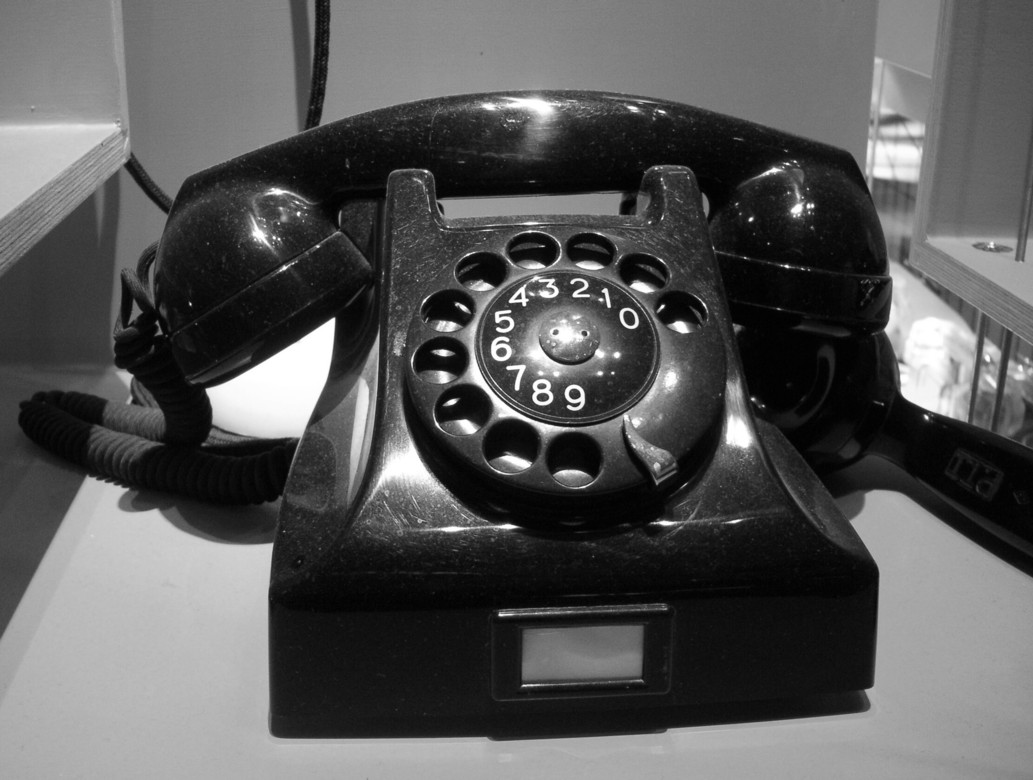
\includegraphics[width=0.42\linewidth]{images/book1/bakelite-telephone.jpg}

{\small Un teléfono de baquelita de 1947. Foto: Holger Ellgaard,
CC BY-SA 3.0.}
\end{omfigure}

\section{Los principales plásticos y sus códigos}

\begin{definition}[Código de identificación de resinas]\label{def:g8:plastics:code}
El \emph{código de identificación de resinas}\index{codigo de identificacion de resinas@código de identificación de resinas}
es un número del 1 al 7, impreso dentro de un triángulo de flechas en un
objeto de \omterm{def:g8:plastics:plastic}{plástico}, que indica de qué \omterm{def:g8:plastics:plastic}{plástico} está hecho, para poder
clasificarlo para el \omterm{def:g5:raw-materials-and-recycling:recycling}{reciclaje}. El triángulo no significa que el objeto
vaya a reciclarse.
\end{definition}

\begin{proposition}[Siete códigos]\label{prop:g8:plastics:codes}
Los códigos, con los usos más corrientes de cada \omterm{def:g8:plastics:plastic}{plástico}:
\begin{center}
\small
\begin{tabular}{cll}
\hline
código & \omterm{def:g8:plastics:plastic}{plástico} & objetos típicos \\
\hline
1 & PET, poli(tereftalato de etileno) & botellas de agua y de refresco, fibras polares \\
2 & PEAD, polietileno de alta densidad & botellas de leche y de champú, tapones \\
3 & PVC, poli(cloruro de vinilo) & tuberías, marcos de ventana, cables \\
4 & PEBD, polietileno de baja densidad & bolsas, películas \\
5 & PP, polipropileno & tarrinas de yogur, tapones, parachoques \\
6 & PS, poliestireno & vasos y bandejas de espuma, cajas de CD \\
7 & otros \omterm{def:g8:plastics:plastic}{plásticos} & \omterm{def:g6:pure-substances-and-mixtures:mixture}{mezclas}, envases multicapa \\
\hline
\end{tabular}
\end{center}
\end{proposition}

\begin{omfigure}
\begin{tikzpicture}[font=\small]
  \foreach \n/\lab in {1/PET, 2/PEAD, 3/PVC, 4/PEBD, 5/PP, 6/PS, 7/OTROS} {
    \begin{scope}[xshift=(\n-1)*2.1cm]
      \foreach \a in {90,210,330} {
        \pgfmathsetmacro\b{\a+120}
        \draw[omDef, line width=1.1pt, ->, >={Stealth[length=4pt]}]
          ($(\a:0.75)!0.14!(\b:0.75)$) -- ($(\a:0.75)!0.86!(\b:0.75)$);
      }
      \node[font=\bfseries] at (0,-0.05) {\n};
      \node[anchor=north, font=\footnotesize] at (0,-0.8) {\lab};
    \end{scope}
  }
\end{tikzpicture}

{\small Los siete \omterm{def:g8:plastics:code}{códigos de identificación de resinas}, cada uno con la
abreviatura de su \omterm{def:g8:plastics:plastic}{plástico}.}
\end{omfigure}

\section{Termoplásticos y termoestables}

\begin{definition}[Termoplástico y termoestable]\label{def:g8:plastics:thermoplastic}
Un \emph{termoplástico}\index{termoplastico@termoplástico} se ablanda cada vez que se
calienta y vuelve a endurecerse al enfriarse: se puede fundir y moldear
una y otra vez (el PET, el polietileno, el PVC, el polipropileno, el
poliestireno). Un \emph{termoestable}\index{termoestable} se endurece
para siempre la primera vez que se calienta y se moldea: si se vuelve a
calentar, no se ablanda, sino que se carboniza (la baquelita, las
resinas de las colas y de los cascos de barco).
\end{definition}

\begin{remark}[Cuáles se pueden reciclar]\label{rem:g8:plastics:which}
Los \omterm{def:g8:plastics:thermoplastic}{termoplásticos} se pueden fundir y volver a moldear: son los
\omterm{def:g8:plastics:plastic}{plásticos} que se reciclan para hacer objetos nuevos. Los \omterm{def:g8:plastics:thermoplastic}{termoestables}
no se pueden volver a fundir.
\end{remark}

\section{Los plásticos en el medio ambiente}

\begin{proposition}[Los plásticos duran]\label{prop:g8:plastics:last}
% ledger: plastics:use-2019, plastics:waste-2019, plastics:recycled-share-2019
En 2019 el mundo consumió unos 460 millones de toneladas de \omterm{def:g8:plastics:plastic}{plásticos} y
tiró unos 353 millones de toneladas de residuos \omterm{def:g8:plastics:plastic}{plásticos}; el \omterm{def:g8:plastics:plastic}{plástico}
\omterm{def:g5:raw-materials-and-recycling:recycling}{reciclado} solo supuso alrededor del \qty{6}{\percent} del \omterm{def:g8:plastics:plastic}{plástico}
utilizado. Los \omterm{def:g8:plastics:plastic}{plásticos} no se pudren: en la naturaleza se rompen en
trozos cada vez más pequeños, los microplásticos, que se encuentran en
los ríos, los océanos, los suelos y el cuerpo de los animales.
\end{proposition}

\begin{omfigure}
\begin{minipage}[t]{0.48\linewidth}\centering
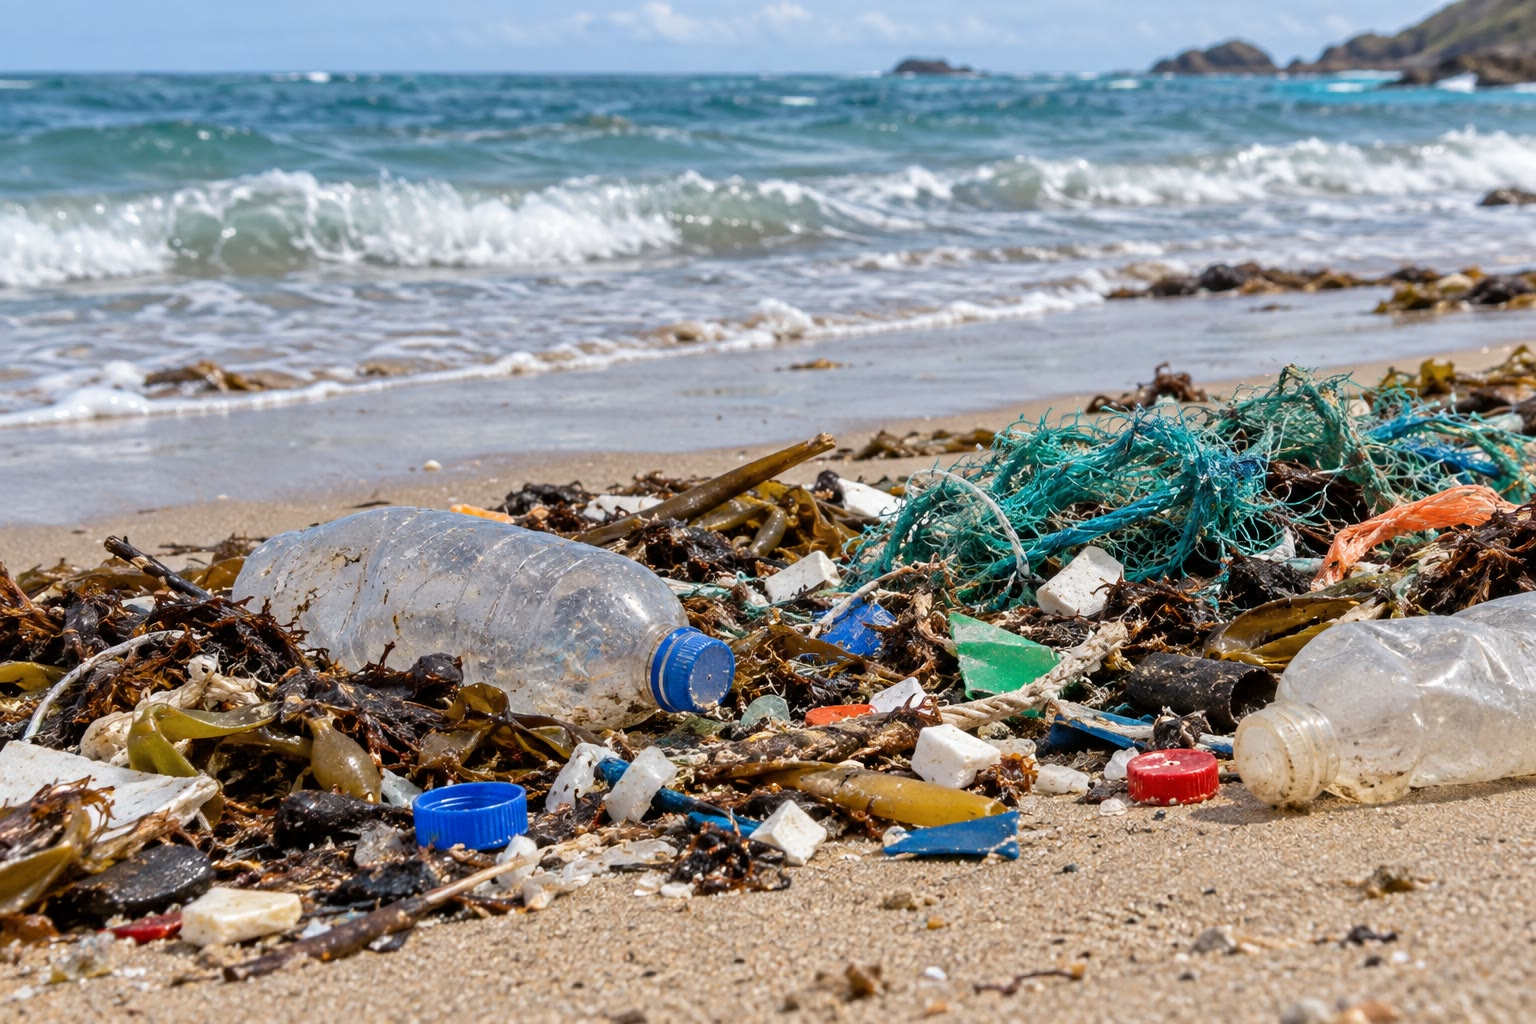
\includegraphics[width=\linewidth,height=4.6cm,keepaspectratio]{images/book1/ai/g8-beach-litter.jpg}

{\small Basura plástica arrastrada hasta una playa.}
\end{minipage}\hfill
\begin{minipage}[t]{0.48\linewidth}\centering
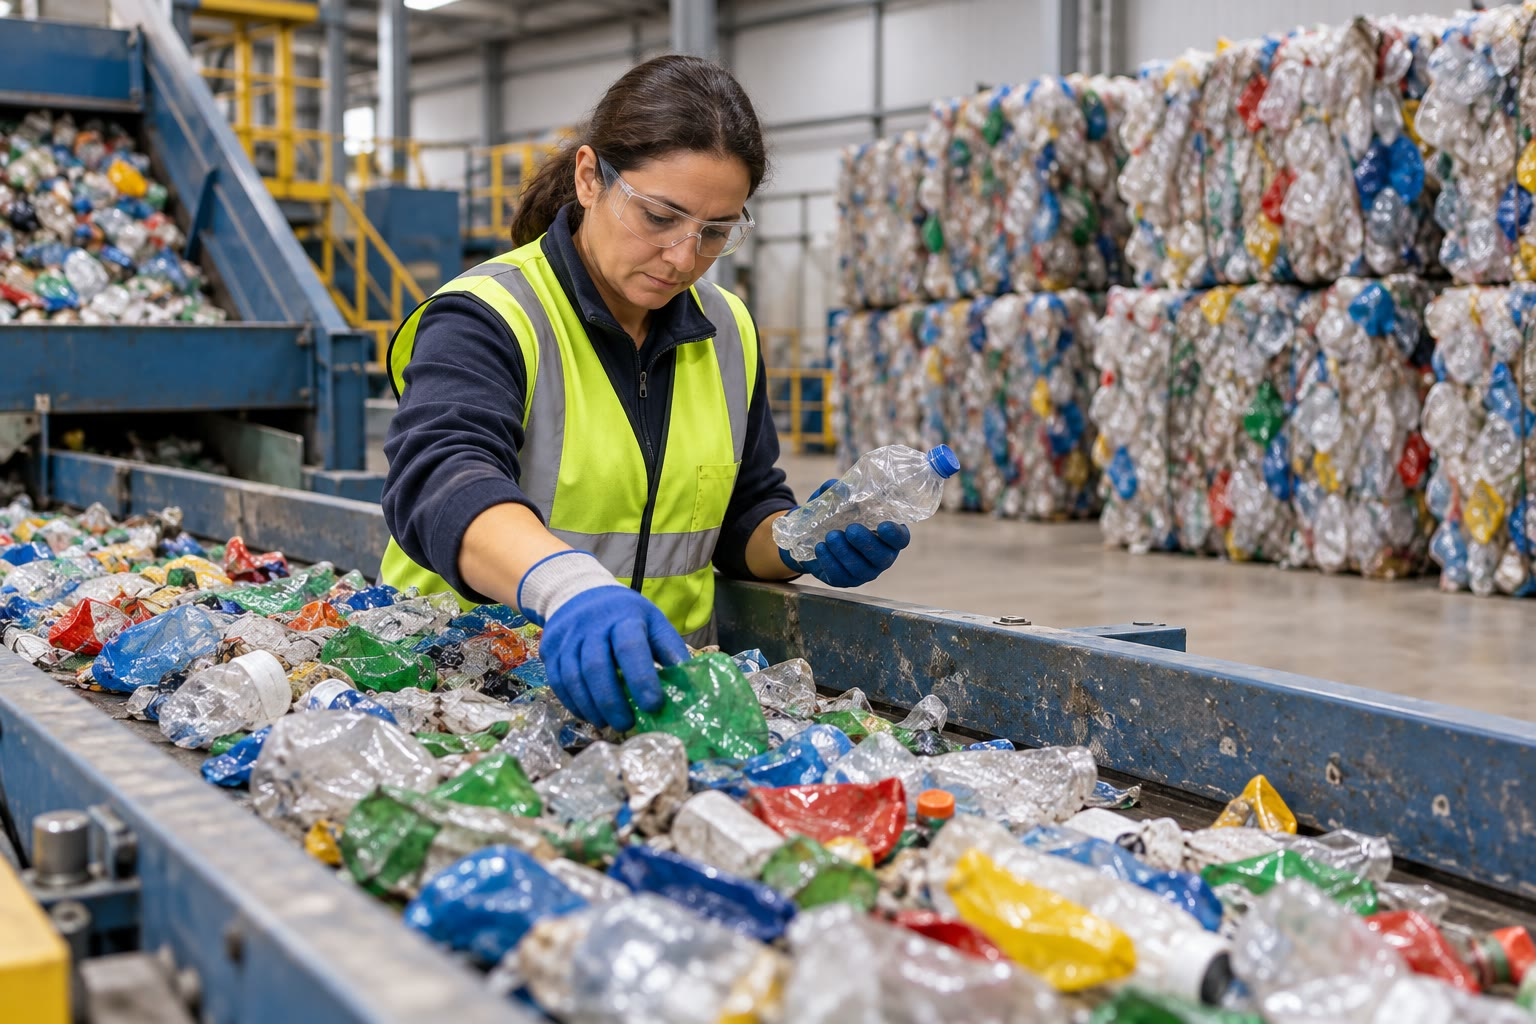
\includegraphics[width=\linewidth,height=4.6cm,keepaspectratio]{images/book1/ai/g8-sorting-line.jpg}

{\small Una línea de clasificación en una planta de \omterm{def:g5:raw-materials-and-recycling:recycling}{reciclaje} de
\omterm{def:g8:plastics:plastic}{plásticos}.}
\end{minipage}
\end{omfigure}

\begin{remark}[Quemar plásticos]\label{rem:g8:plastics:burning}
Los \omterm{def:g8:plastics:plastic}{plásticos} \omterm{def:g4:what-a-fire-needs:burning}{arden}, y producen dióxido de carbono cuando la \omterm{def:g4:what-a-fire-needs:burning}{combustión}
es completa. Pero en una hoguera de jardín \omterm{def:g4:what-a-fire-needs:burning}{arden} de forma incompleta y
liberan hollín, monóxido de carbono y otras sustancias nocivas; el PVC,
que contiene cloro, desprende cloruro de hidrógeno, un gas corrosivo.
Los residuos \omterm{def:g8:plastics:plastic}{plásticos} solo se queman en incineradoras construidas para
depurar sus humos.
\end{remark}

\section{Ejercicios}

\begin{exercise}[$\star$]\label{exo:g8:plastics:1}
¿Natural, artificial o sintético? El algodón, el nailon, el papel, la
lana, el poliestireno, la viscosa.
\end{exercise}

\begin{exercise}[$\star$]\label{exo:g8:plastics:2}
¿A partir de qué \omterm{def:g5:raw-materials-and-recycling:raw-material}{materia prima} se fabrican la mayoría de los \omterm{def:g8:plastics:plastic}{plásticos}?
\end{exercise}

\begin{exercise}[$\star$]\label{exo:g8:plastics:3}
¿Qué \omterm{def:g8:plastics:plastic}{plástico} tiene el código 1? Da un objeto hecho con él.
\end{exercise}

\begin{exercise}[$\star$]\label{exo:g8:plastics:4}
¿Qué diferencia hay entre un \omterm{def:g8:plastics:thermoplastic}{termoplástico} y un \omterm{def:g8:plastics:thermoplastic}{termoestable}?
\end{exercise}

\begin{exercise}[$\star\star$]\label{exo:g8:plastics:5}
Una tarrina de yogur lleva el código 5. Nombra su \omterm{def:g8:plastics:plastic}{plástico} y di si, en
principio, se podría fundir y volver a moldear.
\end{exercise}

\begin{exercise}[$\star\star$]\label{exo:g8:plastics:6}
¿Por qué un triángulo de flechas en un objeto no significa que el objeto
vaya a reciclarse?
\end{exercise}

\begin{exercise}[$\star\star$]\label{exo:g8:plastics:7}
¿Por qué el mango de una sartén suele ser de un \omterm{def:g8:plastics:thermoplastic}{termoestable} y no de un
\omterm{def:g8:plastics:thermoplastic}{termoplástico}?
\end{exercise}

\begin{exercise}[$\star\star$]\label{exo:g8:plastics:8}
Con las cifras de 2019 de este capítulo, ¿qué porcentaje del \omterm{def:g8:plastics:plastic}{plástico}
utilizado se convirtió en residuo ese año? Redondea al número entero más
próximo.
\end{exercise}

\begin{exercise}[$\star\star$]\label{exo:g8:plastics:9}
¿Por qué no hay que quemar nunca PVC en una hoguera de jardín?
\end{exercise}

\begin{exercise}[$\star\star$]\label{exo:g8:plastics:10}
Un instituto usa 300 botellas de \qty{25}{g} cada una por semana,
durante 36 semanas al año. ¿Qué masa de \omterm{def:g8:plastics:plastic}{plástico} es eso en un año?
\end{exercise}

\begin{exercise}[$\star\star\star$]\label{exo:g8:plastics:11}
El polietileno solo está formado por carbono e hidrógeno. Escribe los
productos de su \omterm{def:g8:combustion-and-fuels:complete}{combustión completa}. Explica por qué quemarlo añade
dióxido de carbono al \omterm{def:g4:air-a-mixture-of-gases:air}{aire}, como un \omterm{def:g8:combustion-and-fuels:fossil}{combustible fósil}.
\end{exercise}

\begin{exercise}[$\star\star\star$]\label{exo:g8:plastics:12}
Explica cómo una botella de \omterm{def:g8:plastics:plastic}{plástico} perdida en el mar puede acabar,
años después, convertida en microplásticos dentro de un pez.
\end{exercise}

\section{Problema: La línea de clasificación}

\begin{problem}[{Problema de fin de semana --- una tonelada de botellas
usadas, sus códigos y las escamas de plástico limpias que salen de la
planta}]
\label{pb:g8:plastics:1}
Una planta de \omterm{def:g5:raw-materials-and-recycling:recycling}{reciclaje} recibe balas de botellas de bebida usadas. Una
bala típica de \qty{1}{t} (\qty{1000}{kg}) contiene, en masa: un
\qty{80}{\percent} de cuerpos de botella de PET, un \qty{12}{\percent}
de tapones (PEAD y PP), un \qty{5}{\percent} de etiquetas (película de
PP) y un \qty{3}{\percent} de suciedad y restos de líquido. Unas
máquinas separan los tapones y las etiquetas de los cuerpos, el PET se
tritura en escamas y las escamas se lavan; en el lavado se pierde el
\qty{2.5}{\percent} del PET. Las escamas limpias se funden y se hilan
para hacer las fibras de los forros polares.

\medskip
\noindent\textbf{Parte I --- Los \omterm{def:g8:plastics:plastic}{plásticos}.}
\begin{enumerate}
  \item ¿Qué código está impreso en los cuerpos de las botellas? ¿Y en
        los tapones?
  \item ¿Estos \omterm{def:g8:plastics:plastic}{plásticos} son naturales, artificiales o sintéticos?
  \item ¿Se puede fundir el PET y volver a hilarlo? ¿Qué tipo de
        \omterm{def:g8:plastics:plastic}{plástico} es, por tanto?
  \item ¿Por qué se separan los tapones y las etiquetas de los cuerpos
        antes de fundir el PET?
\end{enumerate}

\medskip
\noindent\textbf{Parte II --- La bala.}
\begin{enumerate}[resume]
  \item ¿Qué masa de PET contiene una bala?
  \item ¿Qué masa de tapones? ¿Y de etiquetas?
  \item ¿Qué masa de la bala no es \omterm{def:g8:plastics:plastic}{plástico}?
  \item ¿Qué porcentaje de la bala es \omterm{def:g8:plastics:plastic}{plástico}?
\end{enumerate}

\medskip
\noindent\textbf{Parte III --- Las escamas.}
\begin{enumerate}[resume]
  \item ¿Qué masa de PET se pierde en el lavado?
  \item Un forro polar necesita \qty{0.39}{kg} de fibra de PET. ¿Por qué
        es mejor fabricarlo con escamas que con PET nuevo?
  \item La planta podría quemar los tapones y las etiquetas para obtener
        calor en lugar de reciclarlos. Nombra el gas que esto añadiría
        al \omterm{def:g4:air-a-mixture-of-gases:air}{aire}.
  \item Calcula la masa de escamas de PET limpias que da una bala.
\end{enumerate}
\end{problem}
